\chapter{Cuerdas, gravedad, compactificación y dualidad T}

\lectureoverview{Una partícula puntual puede moverse de manera coherente en prácticamente cualquier geometría suave, pero una cuerda cuántica no. Sus infinitas oscilaciones de punto cero sondean el espacio objetivo a escalas cada vez menores, y la geometría efectiva cambia a medida que se restituyen esas oscilaciones. Exigir que este proceso tenga un punto fijo conduce a \(R_{\mu\nu}=0\), la ecuación de Einstein en el vacío. Luego pasamos de esta condición de coherencia a la compactificación. Un círculo proporciona tanto estados de momento de Kaluza--Klein como estados de enrollamiento de la cuerda; intercambiarlos identifica un círculo de radio \(R\) con otro de radio \(\alpha'/R\).}

\section{La coherencia como principio de selección}

Hay dos preguntas que responder. ¿Por qué aparece la gravedad en la teoría de cuerdas y por qué esta es mucho menos permisiva que la mecánica de partículas puntuales? En realidad, son una sola pregunta. Una geometría de fondo es admisible únicamente si una cuerda puede propagarse en ella sin conservar una dependencia arbitraria de la resolución con la que la describimos.

Empecemos por el problema de control: una partícula puntual restringida a una superficie curva y suave. Clásicamente, sigue una geodésica, el análogo intrínseco de una línea recta. Se puede aproximar el movimiento mediante muchos segmentos cortos, escribir una ecuación en diferencias y luego hacer tender a cero la longitud de los segmentos. El resultado es una ecuación diferencial ordinaria con un límite continuo bien definido.

La mecánica cuántica modifica la suma sobre historias, pero no la conclusión. En vez de seleccionar una trayectoria clásica, sumamos las amplitudes de las trayectorias sobre la superficie. También aquí se puede dividir el tiempo en pasos pequeños; el límite se describe de forma equivalente mediante una ecuación de Schr\"odinger en el espacio de configuraciones curvo. Para una superficie suave, el límite conduce a un propagador y un espectro definidos.

\begin{figure}[H]
  \centering
  \includegraphics[width=0.72\textwidth]{lecture_09_figure_01.png}
  \caption{Una trayectoria suave sobre la superficie y una trayectoria irregular de la suma cuántica discretizada en el tiempo. Ambas permanecen en la superficie objetivo.}
  \lectureframe{00:05:10}
  \label{fig:l09-particle-paths}
\end{figure}

\begin{classroomqa}
\audiencequestion{En la integral de camino, ¿todas las trayectorias deben permanecer dentro de la superficie? \lecturetimestamp{00:05:39}}
\lecturerresponse{Sí. La superficie es el espacio de configuraciones de la partícula, no una lámina incrustada en una habitación mayor por la que la partícula pueda tomar un atajo. Cada punto intermedio pertenece a la superficie, y todas las longitudes y acciones se calculan con su métrica intrínseca.}
\end{classroomqa}

La pregunta correspondiente para una cuerda es más difícil. Una cuerda no queda especificada solo por la posición de su centro de masa. Tiene una torre infinita de osciladores, de modo que mejorar la resolución significa admitir más grados de libertad dinámicos. La teoría solo es coherente si los observables convergen a un límite al restituir esa torre.

\section{La partícula puntual sobre una esfera}

La esfera es la geometría curva de prueba más sencilla. Sea \(R\) su radio y situemos primero sobre ella una partícula de masa \(m\). Para el movimiento a lo largo de un círculo máximo,
\begin{equation}
  E=\frac{1}{2}mv^2=\frac{p^2}{2m},
  \qquad
  L=pR.
  \label{eq:l09-particle-energy}
\end{equation}
Por consiguiente,
\begin{equation}
  E=\frac{L^2}{2mR^2}
   =\frac{L^2}{2I},
  \qquad
  I=mR^2.
  \label{eq:l09-rotor-energy}
\end{equation}
El radio interviene a través del momento de inercia. Al cuantizar el momento angular se obtiene el conocido espectro del rotor rígido, y nada depende de un corte ultravioleta.

\begin{figure}[H]
  \centering
  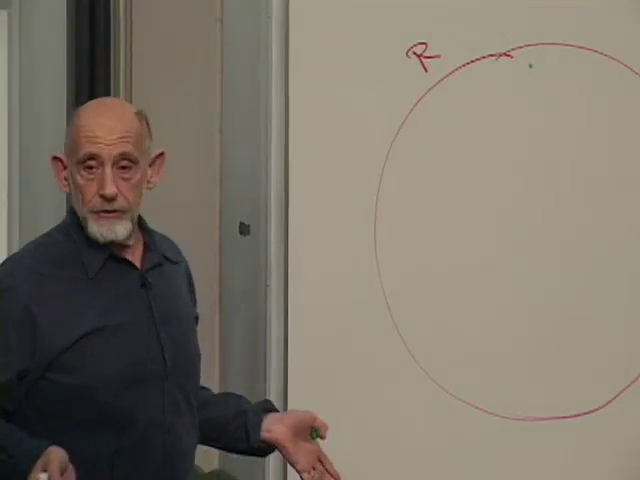
\includegraphics[width=0.74\textwidth]{lecture_09_figure_02.png}
  \caption{El cálculo de control para la partícula puntual:
  \(p^2/(2m)=L^2/(2mR^2)=L^2/(2I)\).}
  \lectureframe{00:11:25}
  \label{fig:l09-sphere-rotor}
\end{figure}

Este ejemplo sin complicaciones es importante. La curvatura por sí sola no es el problema. El problema aparece cuando la curvatura se acopla a la extensión cuántica interna de una cuerda.

\section{La cuerda en el vacío no es puntual}

Consideremos una coordenada transversal de una cuerda abierta y restémosle su centro de masa. La expansión en osciladores que usamos aquí es esquemática:
\begin{equation}
  X(\sigma)-X_{\mathrm{cm}}
  \sim
  \sum_{n=1}^{\infty}
  \frac{a_n+a_n^\dagger}{\sqrt n}\cos(n\sigma).
  \label{eq:l09-mode-expansion}
\end{equation}
Los elementos esenciales son los modos coseno, los operadores de oscilador y el factor \(1/\sqrt n\). Las normalizaciones exactas no influyen en el argumento sobre el tamaño.
\editorialnote{La expansión precisa contiene factores \(\alpha'\) que dependen de las convenciones, constantes numéricas y una elección de notación para los osciladores. La ecuación \eqref{eq:l09-mode-expansion} conserva solo la dependencia necesaria para la estimación ultravioleta, al igual que en la derivación en la pizarra.}

\begin{figure}[H]
  \centering
  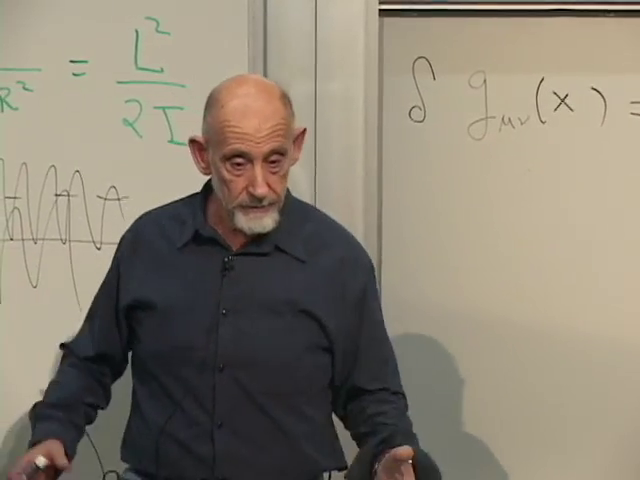
\includegraphics[width=0.78\textwidth]{lecture_09_figure_03.png}
  \caption{La expansión estructural en osciladores y la suma doble que se obtiene al elevarla al cuadrado.}
  \lectureframe{00:15:20}
  \label{fig:l09-string-modes}
\end{figure}

El valor esperado del cuadrado de la distancia al centro de masa en el vacío de osciladores es
\begin{align}
  \expect{\bigl(X(\sigma)-X_{\mathrm{cm}}\bigr)^2}_0
  &\sim
  \sum_{n,m\geq1}
  \frac{\cos(n\sigma)\cos(m\sigma)}{\sqrt{nm}}\notag\\
  &\qquad\times
  \bra{0}(a_n+a_n^\dagger)\notag\\
  &\hspace{6em}\times(a_m+a_m^\dagger)\ket{0}.
  \label{eq:l09-size-double-sum}
\end{align}
La mayoría de los términos se anulan. Dos operadores de aniquilación aniquilan el ket; dos operadores de creación dejan un estado ortogonal al bra; y un operador de creación seguido de uno de aniquilación también tiene valor esperado nulo en el vacío con este orden. La contracción que sobrevive es
\begin{equation}
  \bra{0}a_n a_m^\dagger\ket{0}=\delta_{nm}.
  \label{eq:l09-vacuum-contraction}
\end{equation}

\begin{figure}[H]
  \centering
  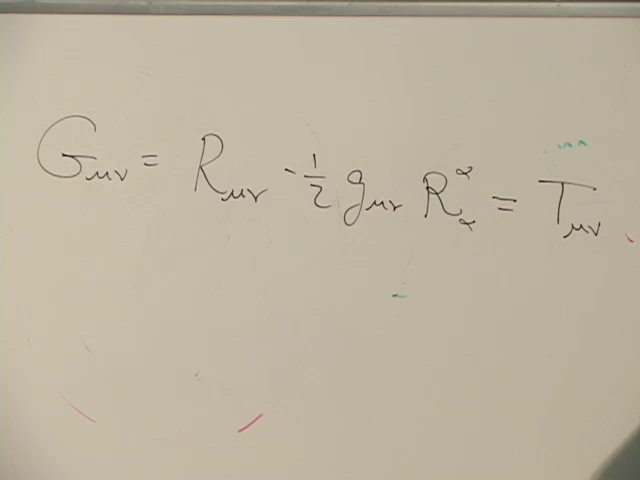
\includegraphics[width=0.74\textwidth]{lecture_09_figure_04.png}
  \caption{La contracción de vacío que sobrevive reduce la suma doble sobre osciladores a una suma simple.}
  \lectureframe{00:20:10}
  \label{fig:l09-vacuum-contraction}
\end{figure}

Así,
\begin{equation}
  \expect{\bigl(X(\sigma)-X_{\mathrm{cm}}\bigr)^2}_0
  \sim
  \sum_{n=1}^{\infty}\frac{\cos^2(n\sigma)}{n}.
  \label{eq:l09-size-single-sum}
\end{equation}
En un punto genérico de la cuerda, o al promediar sobre \(\sigma\), \(\cos^2(n\sigma)\) contribuye aproximadamente \(1/2\). Con un corte en los modos \(N\),
\begin{equation}
  \expect{\bigl(X-X_{\mathrm{cm}}\bigr)^2}_{0,N}
  \sim
  \frac{1}{2}\sum_{n=1}^{N}\frac{1}{n}
  =\frac{1}{2}\log N+O(1).
  \label{eq:l09-logarithmic-size}
\end{equation}

\begin{figure}[H]
  \centering
  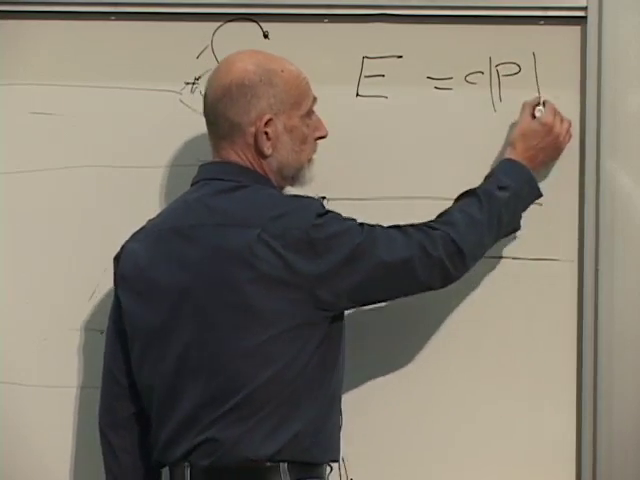
\includegraphics[width=0.72\textwidth]{lecture_09_figure_05.png}
  \caption{En la pizarra se llega a la serie armónica que determina la extensión del estado fundamental.}
  \lectureframe{00:22:05}
  \label{fig:l09-harmonic-size}
\end{figure}

Si se conservan, por ejemplo, solo los primeros veinticinco modos, se obtiene un objeto difuso finito, pero aún no la cuerda continua. Al eliminar el corte, la extensión cuadrática media crece logarítmicamente. No debe interpretarse esta conclusión como una demostración de que la teoría de cuerdas en el espacio plano sea incoherente. En el espacio plano, el movimiento del centro de masa y el de los osciladores se separan, y delicadas cancelaciones en las amplitudes físicas preservan la localidad esperada. El aumento del tamaño es una señal de alerta. La curvatura nos indica si esa señal se convierte en un problema.

\section{Cuando la extensión interna modifica la geometría}

Situemos la cuerda cerca del polo norte de la esfera. Con todos los osciladores apagados, se comporta como la partícula puntual que acabamos de estudiar. A medida que se admiten modos de frecuencia más alta, la cuerda se convierte en un enredo fluctuante que se extiende por el casquete. Su centro puede seguir recorriendo la esfera, pero el objeto cuyo momento de inercia interviene en la energía de rotación ahora tiene extensión.

Para un eje que pasa por el centro de la esfera y por los polos,
\begin{equation}
  I=\int r_\perp^2\,dm,
  \label{eq:l09-extended-inertia}
\end{equation}
donde \(r_\perp\) es la distancia perpendicular entre un elemento de cuerda y ese eje. Un punto del ecuador de la órbita tiene el mayor brazo de palanca pertinente. Las partes de la cuerda que cuelgan hacia el eje contribuyen menos. A masa total fija, esto reduce el momento de inercia efectivo:
\begin{equation}
  I_{\mathrm{eff}}<mR^2.
  \label{eq:l09-inertia-reduction}
\end{equation}
Por tanto, la energía de rotación parece la de un objeto puntual sobre una esfera más pequeña,
\begin{equation}
  E_{\mathrm{rot}}
  =\frac{L^2}{2I_{\mathrm{eff}}}
  \equiv \frac{L^2}{2mR_{\mathrm{eff}}^2},
  \qquad R_{\mathrm{eff}}<R.
  \label{eq:l09-effective-radius}
\end{equation}

\begin{classroomqa}
\audiencequestion{¿Por qué el momento de inercia debería tender a cero si la cuerda se está extendiendo por una región mayor? \lecturetimestamp{00:33:23}}
\lecturerresponse{La afirmación se refiere a la descripción efectiva al efectuar sucesivos promedios a gran escala; no sostiene que la distribución extendida sin promediar tenga de inmediato momento de inercia nulo. La primera banda de modos convierte el punto en una masa difusa que se mueve como si estuviera en una esfera menor. La banda siguiente resuelve la estructura interna de cada una de esas masas y repite la misma renormalización. Al iterar esta comparación, el radio efectivo se reduce.}
\end{classroomqa}

\begin{figure}[H]
  \centering
  \includegraphics[width=0.72\textwidth]{lecture_09_figure_06.png}
  \medskip

  \begin{adjustbox}{max width=\linewidth}
  \begin{tikzpicture}[x=1cm,y=1cm,>=Latex]
    \draw[thick] (0,0) circle (2.15);
    \draw[dashed] (0,-2.55) -- (0,2.55);
    \draw[blue!65!black,thick]
      (-0.22,2.05)
      .. controls (-1.22,1.75) and (-1.52,1.08) .. (-1.06,0.44)
      .. controls (-0.55,-0.10) and (0.35,0.02) .. (1.10,0.68)
      .. controls (1.48,1.12) and (1.16,1.80) .. (0.20,2.05);
    \draw[red!70!black,dashed] (0,0) circle (1.25);
    \draw[->] (2.70,1.55) -- (4.05,1.55);
    \node[align=center] at (3.37,1.98) {add shorter\\modes};
    \draw[thick] (6.15,0) circle (1.25);
    \draw[dashed] (6.15,-1.65) -- (6.15,1.65);
    \draw[blue!65!black,thick]
      (6.00,1.18)
      .. controls (5.42,0.88) and (5.46,0.25) .. (6.02,-0.06)
      .. controls (6.46,-0.28) and (6.90,0.45) .. (6.28,1.18);
    \node at (0,-3.00) {sphere of radius \(R\)};
    \node at (6.15,-2.05) {effective radius \(R_{\mathrm{eff}}\)};
  \end{tikzpicture}
  \end{adjustbox}
\caption{La cuerda cerca del polo norte, tal como aparece en la pizarra, y una reconstrucción clara del argumento del radio efectivo. El círculo interior discontinuo representa una geometría efectiva, no una segunda capa física dentro de la esfera.}
  \lectureframe{00:35:15}
  \label{fig:l09-shrinking-sphere}
\end{figure}

Esto es una afirmación sobre el grupo de renormalización. Con un corte finito, la cuerda es una masa con resolución interna finita. Elevar el corte modifica la mecánica de esa masa. En una esfera de curvatura positiva, cada capa de modos que se añade hace menor el fondo que se infiere a partir del movimiento a larga distancia. Si el resultado nunca se estabiliza, no existe una teoría de cuerdas independiente del corte en ese fondo.

\section{La métrica debe alcanzar un punto fijo}

Sustituyamos ahora la esfera por una métrica general del espacio objetivo \(g_{\mu\nu}(x)\). Integrar una capa logarítmica delgada de modos de oscilador modifica esa métrica mediante un tensor simétrico local de rango dos. La variación debe anularse en el espacio plano y comenzar con dos derivadas de la métrica. A orden dominante, la covariancia deja al tensor de Ricci como candidato pertinente:
\begin{equation}
  \frac{\partial g_{\mu\nu}}{\partial\log\Lambda}
  =-C\,R_{\mu\nu}+\cdots ,
  \qquad C>0
  \label{eq:l09-ricci-flow}
\end{equation}
en el sentido del promedio a gran escala empleado en el argumento geométrico. Así, la curvatura positiva hace que una esfera se contraiga, como se requiere.
\editorialnote{La normalización y el signo dependen de si el parámetro de renormalización aumenta hacia el ultravioleta o hacia el infrarrojo. En la notación convencional de la hoja de universo, la función beta de la métrica a orden dominante es \(\beta^g_{\mu\nu}=\alpha'R_{\mu\nu}+\cdots\). La afirmación invariante que usamos aquí es que la independencia del corte requiere que la función beta, y por tanto \(R_{\mu\nu}\) a este orden, se anule.}

\begin{figure}[H]
  \centering
  \includegraphics[width=0.76\textwidth]{lecture_09_figure_07.png}
  \caption{La variación de la métrica se representa esquemáticamente como menos el tensor de Ricci, junto a una curva que se suaviza.}
  \lectureframe{00:43:00}
  \label{fig:l09-ricci-flow-board}
\end{figure}

\begin{classroomqa}
\audiencequestion{¿Dónde aparece el corte de osciladores \(N\) en esta ecuación de flujo? \lecturetimestamp{00:43:38}}
\lecturerresponse{Es la variable de escala. La suma que determina el tamaño de la cuerda varía logarítmicamente al cambiar el modo de mayor frecuencia incluido, así que el parámetro de evolución natural es \(\log N\), o, de manera equivalente, \(\log\Lambda\). La ecuación \eqref{eq:l09-ricci-flow} describe la variación infinitesimal causada por una capa logarítmica de modos.}
\end{classroomqa}

Un fondo admisible es un punto fijo de este flujo. A orden dominante,
\begin{equation}
  \boxed{R_{\mu\nu}=0.}
  \label{eq:l09-ricci-flat}
\end{equation}
Ser Ricci plano no significa que todas las componentes del tensor de Riemann se anulen. Por ejemplo, las ondas gravitacionales pueden tener curvatura no nula en el vacío y, aun así, satisfacer \(R_{\mu\nu}=0\).

\subsection{La misma condición es la ecuación de Einstein en el vacío}

Con las constantes convencionales suprimidas, la ecuación de Einstein es
\begin{equation}
  G_{\mu\nu}
  \equiv
  R_{\mu\nu}-\frac12 g_{\mu\nu}R
  =T_{\mu\nu}.
  \label{eq:l09-einstein}
\end{equation}

\begin{figure}[H]
  \centering
  \includegraphics[width=0.78\textwidth]{lecture_09_figure_08.png}
  \caption{El tensor de Einstein y el tensor de energía y momento en la pizarra.}
  \lectureframe{00:47:15}
  \label{fig:l09-einstein-board}
\end{figure}

En el vacío, \(T_{\mu\nu}=0\). Tomando la traza en un espacio-tiempo de \(D\) dimensiones se obtiene
\begin{equation}
  0=g^{\mu\nu}G_{\mu\nu}
   =\left(1-\frac{D}{2}\right)R.
  \label{eq:l09-einstein-trace}
\end{equation}
Para \(D\neq2\), \(R=0\), y al sustituir de nuevo en \eqref{eq:l09-einstein} se obtiene \(R_{\mu\nu}=0\). Así, la condición de que la cuerda pierda su dependencia del corte es la ecuación del campo gravitatorio en el vacío. La gravedad no se ha añadido a la teoría; aparece como precio de la coherencia.

La palabra \emph{vacío} no significa que no ocurra nada. Significa que no hay fuentes de energía-momento en la región. Las ecuaciones de Maxwell sin fuentes admiten ondas electromagnéticas, y las ecuaciones de Einstein sin fuentes admiten ondas gravitacionales. La geometría puede ser dinámica aunque su tensor de Ricci se anule.

\begin{classroomqa}
\audiencequestion{¿Está relacionada esta condición con la invariancia conforme?
\lecturetimestamp{00:52:20}}
\lecturerresponse{Sí, aunque la grabación no conserva parte de la pregunta. La simetría pertinente es la invariancia conforme de la teoría cuántica de la \emph{hoja de universo}. Exigir que se anule la anomalía de escala de la hoja de universo es lo que hace que la función beta de la métrica sea cero. No debe confundirse esto con exigir invariancia conforme del propio espacio-tiempo.}
\end{classroomqa}

Hay una segunda condición de coherencia. La invariancia conforme de la hoja de universo también fija la dimensión crítica del espacio-tiempo: diez para las supercuerdas y veintiséis para la cuerda bosónica. Por tanto, la planitud de Ricci no es la lista completa de requisitos, pero sí es la parte que muestra de forma más directa la ecuación de Einstein.

\section{Dimensiones compactas en lugar de dimensiones ausentes}

Un fondo de supercuerdas tiene nueve dimensiones espaciales y una dimensión temporal. Nuestro mundo macroscópico muestra solo tres direcciones espaciales grandes, así que seis dimensiones espaciales deben estar ocultas o ser inaccesibles de algún otro modo a las escalas ordinarias. La compactificación las conserva como direcciones auténticas, pero les asigna una extensión finita pequeña.

\begin{classroomqa}
\audiencequestion{Si distintos observadores llevan relojes distintos, ¿eso equivale a tener más de una dimensión temporal? \lecturetimestamp{00:56:59}}
\lecturerresponse{No. Muchos relojes son muchos instrumentos que miden coordenadas en un solo espacio-tiempo; no crean direcciones temporales independientes. Las dimensiones adicionales que consideramos aquí son espaciales. Las construcciones cuánticas y causales habituales no proporcionan una teoría coherente comparable con varias direcciones temporales locales, así que esa posibilidad no forma parte de este modelo de compactificación.}
\end{classroomqa}

Imaginemos criaturas que creen que su mundo es una línea. A baja resolución, solo pueden moverse hacia delante y hacia atrás. Sin embargo, bajo un microscopio suficientemente potente, se descubre que la línea es un cilindro muy estrecho. Una criatura pequeña puede moverse alrededor de su dirección circular, además de recorrerlo a lo largo. La segunda dirección siempre estuvo presente; su circunferencia era demasiado pequeña para que la detectaran las sondas de baja resolución.

\begin{figure}[H]
  \centering
  \includegraphics[width=0.78\textwidth]{lecture_09_figure_09.png}
  \caption{Un cilindro estrecho y trayectorias que se enrollan alrededor de su dirección circular oculta.}
  \lectureframe{01:01:00}
  \label{fig:l09-hidden-cylinder}
\end{figure}

Un cilindro se puede representar como una franja cuyos bordes superior e inferior están identificados. Al cruzar el borde superior se vuelve por el inferior en la misma posición longitudinal. Ninguno de los bordes es una frontera física. Se puede hacer lo mismo con dos direcciones: se identifican los bordes izquierdo y derecho de un rectángulo, y también sus bordes superior e inferior. El resultado es un toro bidimensional.

\begin{figure}[H]
  \centering
  \includegraphics[width=0.76\textwidth]{lecture_09_figure_10.png}
  \medskip

  \begin{tikzpicture}[x=0.82cm,y=0.82cm,>=Latex]
    \draw[thick] (0,0) rectangle (4,2.15);
    \draw[blue!65!black,->] (0,2.48) -- (4,2.48);
    \draw[blue!65!black,->] (4,-0.34) -- (0,-0.34);
    \node at (2,-0.82) {one periodic direction};
    \draw[thick] (6.1,0) rectangle (10.1,2.15);
    \draw[blue!65!black,->] (6.1,2.48) -- (10.1,2.48);
    \draw[blue!65!black,->] (10.1,-0.34) -- (6.1,-0.34);
    \draw[red!70!black,->] (5.76,0) -- (5.76,2.15);
    \draw[red!70!black,->] (10.44,2.15) -- (10.44,0);
    \node at (8.1,-0.82) {two periodic directions};
  \end{tikzpicture}
  \caption{El prisma de la pizarra y una descripción clara mediante un dominio fundamental. Identificar un par de bordes da un cilindro; identificar ambos pares da un toro.}
  \lectureframe{01:04:40}
  \label{fig:l09-periodic-identification}
\end{figure}

El toro es una topología antes de ser una superficie con forma de rosquilla incrustada en un espacio tridimensional. Si se corta un toro una vez, se convierte en un cilindro; si se vuelve a cortar, se convierte en un rectángulo, siempre que se recuerden las identificaciones de los bordes. Se puede dotar a este rectángulo de una métrica plana; por tanto, el toro plano resultante tiene curvatura de Riemann local nula y, sin duda, es Ricci plano.

Una trayectoria recta en el rectángulo continúa en línea recta al cruzar un borde identificado. Si su pendiente es un cociente racional de los dos períodos, la trayectoria acaba cerrándose. Si el cociente es irracional, nunca se cierra y se vuelve densa en el toro.

\begin{figure}[H]
  \centering
  \includegraphics[width=0.76\textwidth]{lecture_09_figure_11.png}
  \caption{Los segmentos rectos repetidos dentro de un dominio fundamental representan una única trayectoria ininterrumpida sobre el toro.}
  \lectureframe{01:11:00}
  \label{fig:l09-torus-trajectory}
\end{figure}

Los toros de dimensión superior se forman del mismo modo. Un cubo en el que se identifica cada par de caras opuestas es un toro tridimensional, y seis direcciones compactas se pueden modelar mediante un toro de seis dimensiones. No se debe intentar incrustar todos estos objetos en el espacio tridimensional ordinario; la descripción mediante la identificación de caras es intrínseca y completa.

\begin{classroomqa}
\audiencequestion{¿Es necesario que una dimensión adicional se cierre sobre sí misma?
\lecturetimestamp{01:15:03}}
\lecturerresponse{No es un teorema. Podría ser no compacta, pero entonces normalmente aparecería como otra dirección grande en el mundo observado a larga distancia. La compacidad es la forma más sencilla de conciliar las dimensiones adicionales con su aparente ausencia. La razón por la que la naturaleza elige una compactificación concreta es una cuestión dinámica aparte.}
\end{classroomqa}

\begin{classroomqa}
\audiencequestion{¿Por qué suponer que las dimensiones que no vemos son direcciones espaciales ordinarias enrolladas de esta manera y no algo completamente distinto? \lecturetimestamp{01:15:51}}
\lecturerresponse{Porque es una hipótesis concreta y resoluble, no porque se haya demostrado que sea la única descripción de la naturaleza. Las variedades espaciales compactas nos permiten construir ejemplos coherentes y calcular sus espectros. Las posibilidades más exóticas deben demostrar que también pueden hacerlo.}
\end{classroomqa}

\begin{classroomqa}
\audiencequestion{Las distancias en el toro familiar con forma de rosquilla no parecen distancias en un rectángulo. ¿A qué geometría nos referimos?
\lecturetimestamp{01:18:11}}
\lecturerresponse{El término \emph{toro} fija las identificaciones, no una métrica única. La rosquilla incrustada hereda una métrica curva del espacio tridimensional. El rectángulo con identificaciones periódicas tiene una métrica plana. Tienen la misma topología y geometrías distintas; para la compactificación sencilla nos referimos a la plana.}
\end{classroomqa}

\section{Los parámetros de forma de un toro plano}

Ni siquiera un toro plano bidimensional es único. Su paralelogramo fundamental tiene un área total, una razón de aspecto y un sesgo. Cambiar estos parámetros modifica las distancias y, por tanto, el espectro, sin cambiar la topología.

\begin{figure}[H]
  \centering
  \includegraphics[width=0.74\textwidth]{lecture_09_figure_12.png}
  \medskip

  \begin{tikzpicture}[x=0.9cm,y=0.9cm,>=Latex]
    \draw[thick] (0,0) rectangle (3.4,2.1);
    \draw[<->] (0,-0.35) -- node[below] {\(L_1\)} (3.4,-0.35);
    \draw[<->] (-0.35,0) -- node[left] {\(L_2\)} (-0.35,2.1);
    \draw[thick] (5.4,0) -- (8.8,0) -- (9.7,2.1) -- (6.3,2.1) -- cycle;
    \draw[dashed] (5.4,0) -- (6.3,2.1);
    \draw[->] (5.75,2.48) -- node[above] {shear} (6.45,2.48);
    \node at (1.7,-1.00) {area and aspect ratio};
    \node at (7.55,-1.00) {complex structure};
  \end{tikzpicture}
  \caption{Los dominios fundamentales rectangular y sesgado que se usan para analizar los módulos del toro.}
  \lectureframe{01:23:00}
  \label{fig:l09-torus-moduli}
\end{figure}

Para un toro bidimensional, resulta útil representar la forma mediante un número complejo \(\tau=\tau_1+i\tau_2\): la parte real registra el sesgo y la parte imaginaria, la razón de aspecto una vez separado el factor de escala global. Intercambiar los dos ciclos básicos o cambiar su base entera puede hacer que paralelogramos aparentemente diferentes describan el mismo toro.

\begin{classroomqa}
\audiencequestion{¿Qué ocurre si se invierte un borde antes de identificarlo? \lecturetimestamp{01:24:20}}
\lecturerresponse{Eso produce una topología distinta. Identificar mediante una reflexión da lugar a una superficie no orientable, la botella de Klein, en vez de un toro ordinario.}
\end{classroomqa}

\begin{classroomqa}
\audiencequestion{¿Qué ocurre si el giro no es uniforme a lo largo del borde?
\lecturetimestamp{01:25:01}}
\lecturerresponse{Una deformación suave no uniforme se puede incorporar a la métrica del dominio fundamental. Hay que mantener diferenciadas la identificación topológica y los datos geométricos: cambiar la unión puede modificar la topología, mientras que cambiar suavemente las distancias modifica la métrica.}
\end{classroomqa}

\editorialnote{Para un toro plano bidimensional, el área es el módulo de Kähler más sencillo y \(\tau\) es el módulo de la estructura compleja. Un sesgo continuo forma parte de \(\tau\). En cambio, un giro de Dehn es una operación discreta de clase de mapeo, representada por \(\tau\mapsto\tau+1\); no es en sí mismo el módulo continuo. Esto precisa la terminología intencionadamente informal usada durante la discusión en la pizarra.}

Los toros planos son útiles porque satisfacen inmediatamente la condición de coherencia, pero su simetría es demasiado amplia para un modelo realista de física de partículas. Espacios Ricci planos más complejos, en particular las variedades de Calabi--Yau, dan lugar a compactificaciones más ricas. Su construcción detallada queda fuera de esta discusión; el principio es el mismo.

\section{Leer un círculo compacto a partir de su espectro}

Después del descanso, reduzcamos el espacio compacto a un círculo de circunferencia \(2\pi R\). La función de onda debe ser monovaluada después de una vuelta:
\begin{equation}
  e^{ip_c(x+2\pi R)/\hbar}=e^{ip_cx/\hbar}.
\end{equation}
Por tanto,
\begin{equation}
  p_cR=n\hbar,
  \qquad
  p_c=\frac{n\hbar}{R},
  \qquad n\in\mathbb Z.
  \label{eq:l09-kk-momentum}
\end{equation}

\begin{figure}[H]
  \centering
  \includegraphics[width=0.74\textwidth]{lecture_09_figure_13.png}
  \caption{La circunferencia compacta \(2\pi R\) y el momento cuantizado \(p_c=n\hbar/R\).}
  \lectureframe{01:32:15}
  \label{fig:l09-kk-board}
\end{figure}

Para una partícula sin masa en el espacio-tiempo completo,
\begin{equation}
  E=c|\mathbf P|.
  \label{eq:l09-massless-dispersion}
\end{equation}

\begin{figure}[H]
  \centering
  \includegraphics[width=0.70\textwidth]{lecture_09_figure_14.png}
  \caption{La relación de dispersión de la partícula sin masa, usada para reinterpretar el momento compacto como masa en menos dimensiones.}
  \lectureframe{01:33:45}
  \label{fig:l09-massless-board}
\end{figure}

Separemos el momento en sus partes no compacta y compacta, y fijemos \(c=\hbar=1\):
\begin{equation}
  E^2=\mathbf p_{\mathrm{large}}^2+\frac{n^2}{R^2}.
  \label{eq:l09-kk-dispersion}
\end{equation}
Un observador que no puede resolver la dirección compacta compara esto con \(E^2=\mathbf p_{\mathrm{large}}^2+m^2\) e infiere una torre de masas:
\begin{equation}
  m_n=\frac{|n|}{R}.
  \label{eq:l09-kk-masses}
\end{equation}
Los dos signos de \(n\) describen momentos compactos opuestos con la misma energía positiva, no masas positivas y negativas. Por tanto, el espaciamiento \(1/R\) permite determinar el radio mediante espectroscopia. Este es el mecanismo de Kaluza--Klein: el momento en una dirección oculta aparece como masa en las dimensiones visibles.

\section{Los estados de enrollamiento completan el espectro}

Una cuerda cerrada tiene una posibilidad que no tiene una partícula puntual: puede dar vueltas alrededor del círculo. Si el número de enrollamiento es \(w\), la cuerda solo se cierra después de recorrer la dirección compacta \(w\) veces. Su longitud es \(2\pi |w|R\), así que la tensión aporta una energía de
\begin{equation}
  m_w
  =2\pi T\,|w|R
  =\frac{|w|R}{\alpha'}.
  \label{eq:l09-winding-mass}
\end{equation}
La lección elige unidades con \(\alpha'=1\), con lo que se reduce a
\begin{equation}
  m_w=|w|R.
  \label{eq:l09-winding-lecture-units}
\end{equation}
Los valores positivo y negativo de \(w\) corresponden a orientaciones opuestas alrededor del círculo.

\begin{figure}[H]
  \centering
  \includegraphics[width=0.76\textwidth]{lecture_09_figure_15.png}
  \caption{Una cuerda cerrada enrollada alrededor del cilindro compacto, cuyo radio compacto está indicado en la pizarra.}
  \lectureframe{01:39:45}
  \label{fig:l09-winding-board}
\end{figure}

Así pues, el círculo compacto da lugar a dos torres complementarias:
\begin{equation}
  m_n=\frac{|n|}{R},
  \qquad
  m_w=\frac{|w|R}{\alpha'}.
  \label{eq:l09-two-towers}
\end{equation}
Cuando \(R\) es grande, los niveles de momento están muy próximos y los estados de enrollamiento son pesados. Cuando \(R\) es pequeño, los niveles de momento están muy separados y los estados de enrollamiento son ligeros.

\begin{figure}[H]
  \centering
  \begin{tikzpicture}[x=1cm,y=0.9cm,>=Latex]
    \draw[->] (0,0) -- (0,4.7) node[above] {\(m\)};
    \foreach \y/\lab in {0/0,1.1/{1/R},2.2/{2/R},3.3/{3/R},4.4/{4/R}} {
      \draw (-0.16,\y) -- (0.16,\y);
      \node[left] at (-0.22,\y) {\(\lab\)};
    }
    \node at (0,-0.62) {momentum};
    \draw[<->,very thick,blue!65!black] (2.05,2.15) -- (4.05,2.15)
      node[midway,above] {\(R\leftrightarrow\alpha'/R\)};
    \draw[->] (6.1,0) -- (6.1,4.7) node[above] {\(m\)};
    \foreach \y/\lab in {0/0,1.1/{R/\alpha'},2.2/{2R/\alpha'},3.3/{3R/\alpha'},4.4/{4R/\alpha'}} {
      \draw (5.94,\y) -- (6.26,\y);
      \node[right] at (6.32,\y) {\(\lab\)};
    }
    \node at (6.1,-0.62) {winding};
  \end{tikzpicture}
  \caption{Las torres de momento y de enrollamiento se intercambian al invertir el radio en unidades de cuerda.}
  \label{fig:l09-dual-mass-towers}
\end{figure}

\section{Dualidad T: los círculos pequeños y grandes describen la misma física}

Las dos torres se intercambian mediante
\begin{equation}
  R\longleftrightarrow\frac{\alpha'}{R},
  \qquad
  n\longleftrightarrow w.
  \label{eq:l09-t-duality}
\end{equation}
En las unidades usadas en la pizarra, \(\alpha'=1\), así que esto se reduce a \(R\leftrightarrow1/R\). En el radio autodual \(R=\sqrt{\alpha'}\), coinciden las escalas de momento y de enrollamiento.

\begin{figure}[H]
  \centering
  \includegraphics[width=0.74\textwidth]{lecture_09_figure_16.png}
  \caption{En la pizarra se comparan las escaleras de masas, más dispersa y más densa, a medida que el radio atraviesa la escala autodual.}
  \lectureframe{01:43:00}
  \label{fig:l09-duality-board}
\end{figure}

El intercambio de las fórmulas elementales de las masas es solo el aspecto más visible del resultado. Los estados de oscilador de la cuerda cerrada y las amplitudes de dispersión también se transforman de manera coherente. Un círculo menor que la escala de cuerda no constituye una geometría nueva, cada vez más diminuta; tiene una descripción equivalente mediante un círculo dual mayor. Las partículas puntuales no pueden establecer esta identificación porque tienen modos de momento, pero no modos de enrollamiento.

\begin{classroomqa}
\audiencequestion{¿Es simplemente lo mismo que intercambiar una dirección vertical por una horizontal? \lecturetimestamp{01:44:38}}
\lecturerresponse{No. Se intercambian dos números cuánticos distintos: el momento alrededor del círculo y el número de veces que una cuerda cerrada lo recorre. Al mismo tiempo, hay que invertir el radio.}
\end{classroomqa}

\begin{classroomqa}
\audiencequestion{¿Las descripciones en \(R<\sqrt{\alpha'}\) y \(R>\sqrt{\alpha'}\) se refieren solo a bosones o también a fermiones?
\lecturetimestamp{01:46:30}}
\lecturerresponse{La dualidad es una simetría de toda la teoría de cuerdas compactificada, no solo de la sencilla escalera bosónica de masas que hemos usado para ponerla de manifiesto. El detalle de la correspondencia entre sectores depende de la teoría, pero la equivalencia entre radios pequeños y grandes no se restringe a una especie de partícula.--
}
\end{classroomqa}

\begin{classroomqa}
\audiencequestion{¿Los dos estados que se comparan son cuerdas abiertas o cerradas? \lecturetimestamp{01:47:32}}
\lecturerresponse{Son estados de cuerda cerrada. Una cuerda cerrada que se propaga libremente puede enrollarse alrededor de un círculo compacto. Una cuerda abierta ordinaria con extremos libres no tiene el mismo número de enrollamiento conservado.}
\end{classroomqa}
\editorialnote{En el tratamiento más completo de las cuerdas abiertas, la dualidad T intercambia las condiciones de contorno de Neumann y Dirichlet e introduce las D-branas. Por eso la dualidad T para cuerdas abiertas es más rica que una simple reproducción de la fórmula de enrollamiento para cuerdas cerradas.}

\begin{classroomqa}
\audiencequestion{¿Es este intercambio análogo al intercambio entre espacio y tiempo cerca del horizonte de un agujero negro? \lecturetimestamp{01:48:00}}
\lecturerresponse{No. Las coordenadas del horizonte y el carácter causal plantean una cuestión distinta. Aquí las dos descripciones se refieren a un único círculo espacial compacto y al intercambio de sus sectores de momento y enrollamiento.}
\end{classroomqa}

\begin{classroomqa}
\audiencequestion{¿Esto resuelve el problema de la autoenergía a distancias cortas al proporcionar una longitud mínima? \lecturetimestamp{01:48:35}}
\lecturerresponse{Muestra que los radios menores que la escala de cuerda no definen fondos de círculo nuevos e inequivalentes: al disminuir \(R\) más allá del punto autodual, aumenta el radio dual. Esto supone un impedimento preciso propio de las cuerdas para sondear una geometría circular arbitrariamente pequeña, aunque no debe transformarse en la afirmación de que toda noción imaginable de distancia tenga un único límite inferior rígido y universal.}
\end{classroomqa}

\section{Por qué no se pueden omitir los sectores de enrollamiento}

\begin{classroomqa}
\audiencequestion{¿Podríamos definir la teoría usando solo cuerdas no enrolladas y
prescindir de los estados de enrollamiento? \lecturetimestamp{01:48:56}}
\lecturerresponse{No. Las interacciones de cuerdas cerradas los generan. Estirad
un lazo no enrollado alrededor de la dirección compacta, de modo que un segmento siga
el círculo en un sentido y otro lo recorra en el sentido opuesto. El enrollamiento
neto sigue siendo cero. Después, una reconexión puede dividir el lazo en dos
cuerdas cerradas con enrollamientos \(+1\) y \(-1\). El par puede separarse, así que
los estados de enrollamiento deben formar parte del espectro incluso si el estado
inicial no contenía ninguno.}
\end{classroomqa}

\begin{figure}[H]
  \centering
  \includegraphics[width=0.74\textwidth]{lecture_09_figure_17.png}
  \caption{El lazo no enrollado, estirado y dispuesto alrededor de la dirección
  compacta antes de la reconexión.}
  \lectureframe{01:50:30}
  \label{fig:l09-winding-pair-before}
\end{figure}

\begin{figure}[H]
  \centering
  \includegraphics[width=0.72\textwidth]{lecture_09_figure_18.png}
  \medskip

  \begin{tikzpicture}[x=0.9cm,y=0.9cm,>=Latex]
    \draw[thick] (0,0) ellipse (1.0 and 1.55);
    \draw[blue!65!black,thick]
      (0.08,1.35) .. controls (2.0,1.15) and (2.0,-1.15) .. (0.08,-1.35);
    \draw[red!70!black,thick]
      (-0.08,-1.35) .. controls (-2.0,-1.15) and (-2.0,1.15) .. (-0.08,1.35);
    \node at (0,-2.15) {net \(w=0\)};
    \draw[->,thick] (2.45,0) -- (3.75,0) node[midway,above] {split};
    \draw[thick] (5.05,0.62) ellipse (0.68 and 1.02);
    \draw[blue!65!black,very thick,->]
      (5.05,1.64) arc[start angle=90,end angle=-250,x radius=0.68,y radius=1.02];
    \node at (5.05,-0.82) {\(w=+1\)};
    \draw[thick] (7.45,0.62) ellipse (0.68 and 1.02);
    \draw[red!70!black,very thick,<-]
      (7.45,1.64) arc[start angle=90,end angle=-250,x radius=0.68,y radius=1.02];
    \node at (7.45,-0.82) {\(w=-1\)};
  \end{tikzpicture}
  \caption{El bucle con enrollamiento separado en la pizarra y una reconstrucción limpia de la producción de pares de enrollamiento--antienrollamiento. El enrollamiento total sigue siendo cero.}
  \lectureframe{01:51:30}
  \label{fig:l09-winding-pair-after}
\end{figure}

\begin{classroomqa}
\audiencequestion{¿Producir el par de estados de enrollamiento requiere energía adicional?
\lecturetimestamp{01:52:11}}
\lecturerresponse{Sí. Estirar una cuerda requiere energía de tensión, y las
cuerdas enrolladas finales tienen las masas indicadas en
\eqref{eq:l09-winding-mass}. Una colisión con energía suficiente puede
producir el par, del mismo modo que una colisión puede producir una partícula y su
antipartícula, conservando la carga conservada pertinente.}
\end{classroomqa}

\section{¿Se puede oír la forma de un fondo de cuerdas?}

En una teoría ordinaria de partículas compactificada, el espaciado del
espectro de Kaluza--Klein permite inferir el radio: se intenta oír la forma
del espacio compacto a partir de sus modos normales. La teoría de cuerdas hace más sutil el
problema inverso. Los modos de momento detectan \(1/R\), los modos de enrollamiento detectan
\(R/\alpha'\), y el espectro completo no cambia al intercambiarlos. Dos radios que la geometría
para partículas puntuales considera distintos corresponden a un mismo fondo de cuerdas
descrito mediante variables duales.

Así, la lección ha llegado por una misma vía a las dos conclusiones que había anunciado.
La consistencia ultravioleta obliga a que la métrica del espacio objetivo satisfaga la
ecuación de Einstein en el vacío, de modo que la gravedad es inevitable. La
compactificación convierte entonces la geometría oculta en espectros de partículas, pero los
estados de enrollamiento impiden que ese espectro determine un radio clásico único por debajo
de la escala de cuerdas. La consistencia no solo selecciona qué geometrías están permitidas:
a través de la dualidad T, cambia también qué se considera una geometría distinta.